%%%%%%%%%%%%%%%%%%%%%%%%%%%%%%%%%%%%%%%%%
% a0poster Portrait Poster
% LaTeX Template
% Version 1.0 (22/06/13)
%%%%%%%%%%%%%%%%%%%%%%%%%%%%%%%%%%%%%%%%%

\documentclass[a0,portrait]{a0poster}

\usepackage{multicol}
\columnsep=100pt
\columnseprule=3pt

\usepackage[svgnames]{xcolor}

\usepackage{tabularx} % Defines the tabularx environment and X column
\usepackage{booktabs} % Defines \toprule, \midrule, and \bottomrule

% --- BIBLIOGRAPHY SETUP ---
\usepackage[style=authoryear, backend=biber, maxcitenames=2]{biblatex}
\addbibresource{references.bib} % Your bibliography file

% Make the bibliography font smaller to save space
\renewcommand*{\bibfont}{\small}

% OFFICIAL UNIVERSITY OF COLOGNE COLOR DEFINITION
\definecolor{UoCBlue}{RGB}{0, 51, 102}
\definecolor{UoCGray}{RGB}{119, 119, 119}

\usepackage{times}
\usepackage{graphicx}
\graphicspath{{../../Results/Figures/}}

\usepackage{booktabs}
\usepackage[font=small,labelfont=bf]{caption}
\usepackage{amsfonts, amsmath, amsthm, amssymb}
\usepackage{wrapfig}

\usepackage[most]{tcolorbox}
\usepackage{enumitem}
\usepackage{setspace}
\onehalfspacing


\tcbset{
  presentbox/.style={
    colback=white,
    fonttitle=\bfseries,
    toptitle=8pt,
    bottomtitle=8pt,
    top=10pt, bottom=10pt,
    left=10pt, right=10pt,
  }
}


\begin{document}

%----------------------------------------------------------------------------------------
%   POSTER HEADER
%----------------------------------------------------------------------------------------

\begin{minipage}[b]{0.68\linewidth}
\Huge \color{UoCBlue} \textbf{Sparse Learning and Endogenous Pockets of Predictability} \color{Black}\\[2cm]
\huge \textbf{\color{UoCBlue} Tommaso Di Francesco, Stefanie Huber, \& Jonathan Seim}\\[0.5cm]
\huge University of Bonn \& University of Cologne \\[0.4cm]
\Large April 14, 2026\\
\end{minipage}%
\begin{minipage}[b]{0.30\linewidth}
\raggedleft
\includegraphics[width=18cm]{"Universitaet zu Koeln Logo ENG"}
\end{minipage}


\begin{multicols*}{2}

%----------------------------------------------------------------------------------------
%   ABSTRACT
%----------------------------------------------------------------------------------------

\color{UoCBlue}
\section*{Abstract}
\color{Black}

This paper studies the implications for financial markets when investors increasingly use machine learning to search for return predictability.
We study an asset-pricing model in which agents believe that some set of observable signals are linearly related to realised returns.
As the number of signals exceeds the number of observations agents have, we endow them with a novel learning mechanism called \textit{LASSO learning}.
Under this rule, agents first estimate the least squares estimate for each signal, but then only retain those signals whose coefficient exceeds a certain threshold.
This learning rule enforces sparsity and thereby enables agents to consider a large number of signals when making forecasts.
Our main result is that the search for predictability endogenously generates episodes of true return predictability.
% This holds even when returns are driven by an unpredictable fundamental process.
Return predictability arises through a feedback mechanism between agents' return expectations, as implied by their LASSO estimates, and realized returns.
We demonstrate the empirical relevance of the model in the cross-section of U.S. stock returns.


\vspace{0.5cm}



%----------------------------------------------------------------------------------------
%   THE MODEL
%----------------------------------------------------------------------------------------

\begin{tcolorbox}[colback=white, colframe=UoCBlue, title=Environment and Benchmark, toptitle=10pt, bottomtitle=10pt, fonttitle=\bfseries]

\vspace{0.5cm}
We study a standard \textcite{lucas1978} asset-pricing model where a continuum of agents trades a single risky asset that pays a stochastic dividend $D_t$.  \\
The equilibrium price of the asset is determined by the standard no-arbitrage condition:
\begin{equation}\label{eq:equilibrium_price}
    P_t = \delta \mathbb{E}_t \left[ \left(\frac{C_{t+1}}{C_t}\right)^{- \ell} P_{t+1} + D_{t+1} \right]
\end{equation}

\vspace{0.5cm}
Under full information rational expectations (FIRE), the price-dividend ratio is constant. Returns are driven entirely by fundamental dividend shocks and are therefore unpredictable:
\begin{equation}
    r_{t+1} = \log(a) + \eta_{t+1}^{d} \sim \mathcal{N}(\log(a) - \sigma_{d}^{2}/2, \sigma_{d}^{2})
\end{equation}

\vspace{0.5cm}
\end{tcolorbox}







\begin{tcolorbox}[colback=white,colframe=UoCBlue, title = Bounded Rationality and LASSO Learning, toptitle=10pt, bottomtitle=10pt, fonttitle=\bfseries]

\vspace{0.5cm}
We follow \textcite{adam2016stock} and assume agents know the processes for dividends and consumption but are boundedly rational with respect to returns.
They suspect returns are conditionally predictable from a high-dimensional set of observable signals $x_t$.
In the model, agents belief in a linear \textbf{Perceived Law of Motion (PLM)} for returns:

\vspace{0.05cm}
\begin{equation}
    r_{t+1} = x_{t}\beta + u_{t+1}
\end{equation}
\vspace{0.05cm}

Because the number of candidate predictors exceeds the sample size, agents cannot estimate all coefficients simultaneously.
Instead, they estimate the PLM through \textbf{LASSO learning}.
First, they estimate OLS coefficients for each predictor.
Then, they apply a soft-thresholding rule to shrink small coefficients to exactly zero:

\vspace{0.05cm}
\begin{equation}
     \beta^{LASSO}_t = \text{sign}(\beta^{OLS}_t)\max\{0, |\beta^{OLS}_t| - \lambda\}
\end{equation}
\vspace{0.05cm}

When a signal is strong enough, agents trade on this perceived predictability, and their demand feeds back into prices. This process makes the \textbf{Actual Law of Motion (ALM)} nonlinear:

\vspace{0.05cm}
\begin{equation}
    r_{t+1} = \log(1 - \kappa e^{x_{t}\beta}) - \log(1 - \kappa e^{x_{t+1}\beta}) + \eta_{t+1}
\end{equation}
\vspace{0.05cm}

\begin{center}
    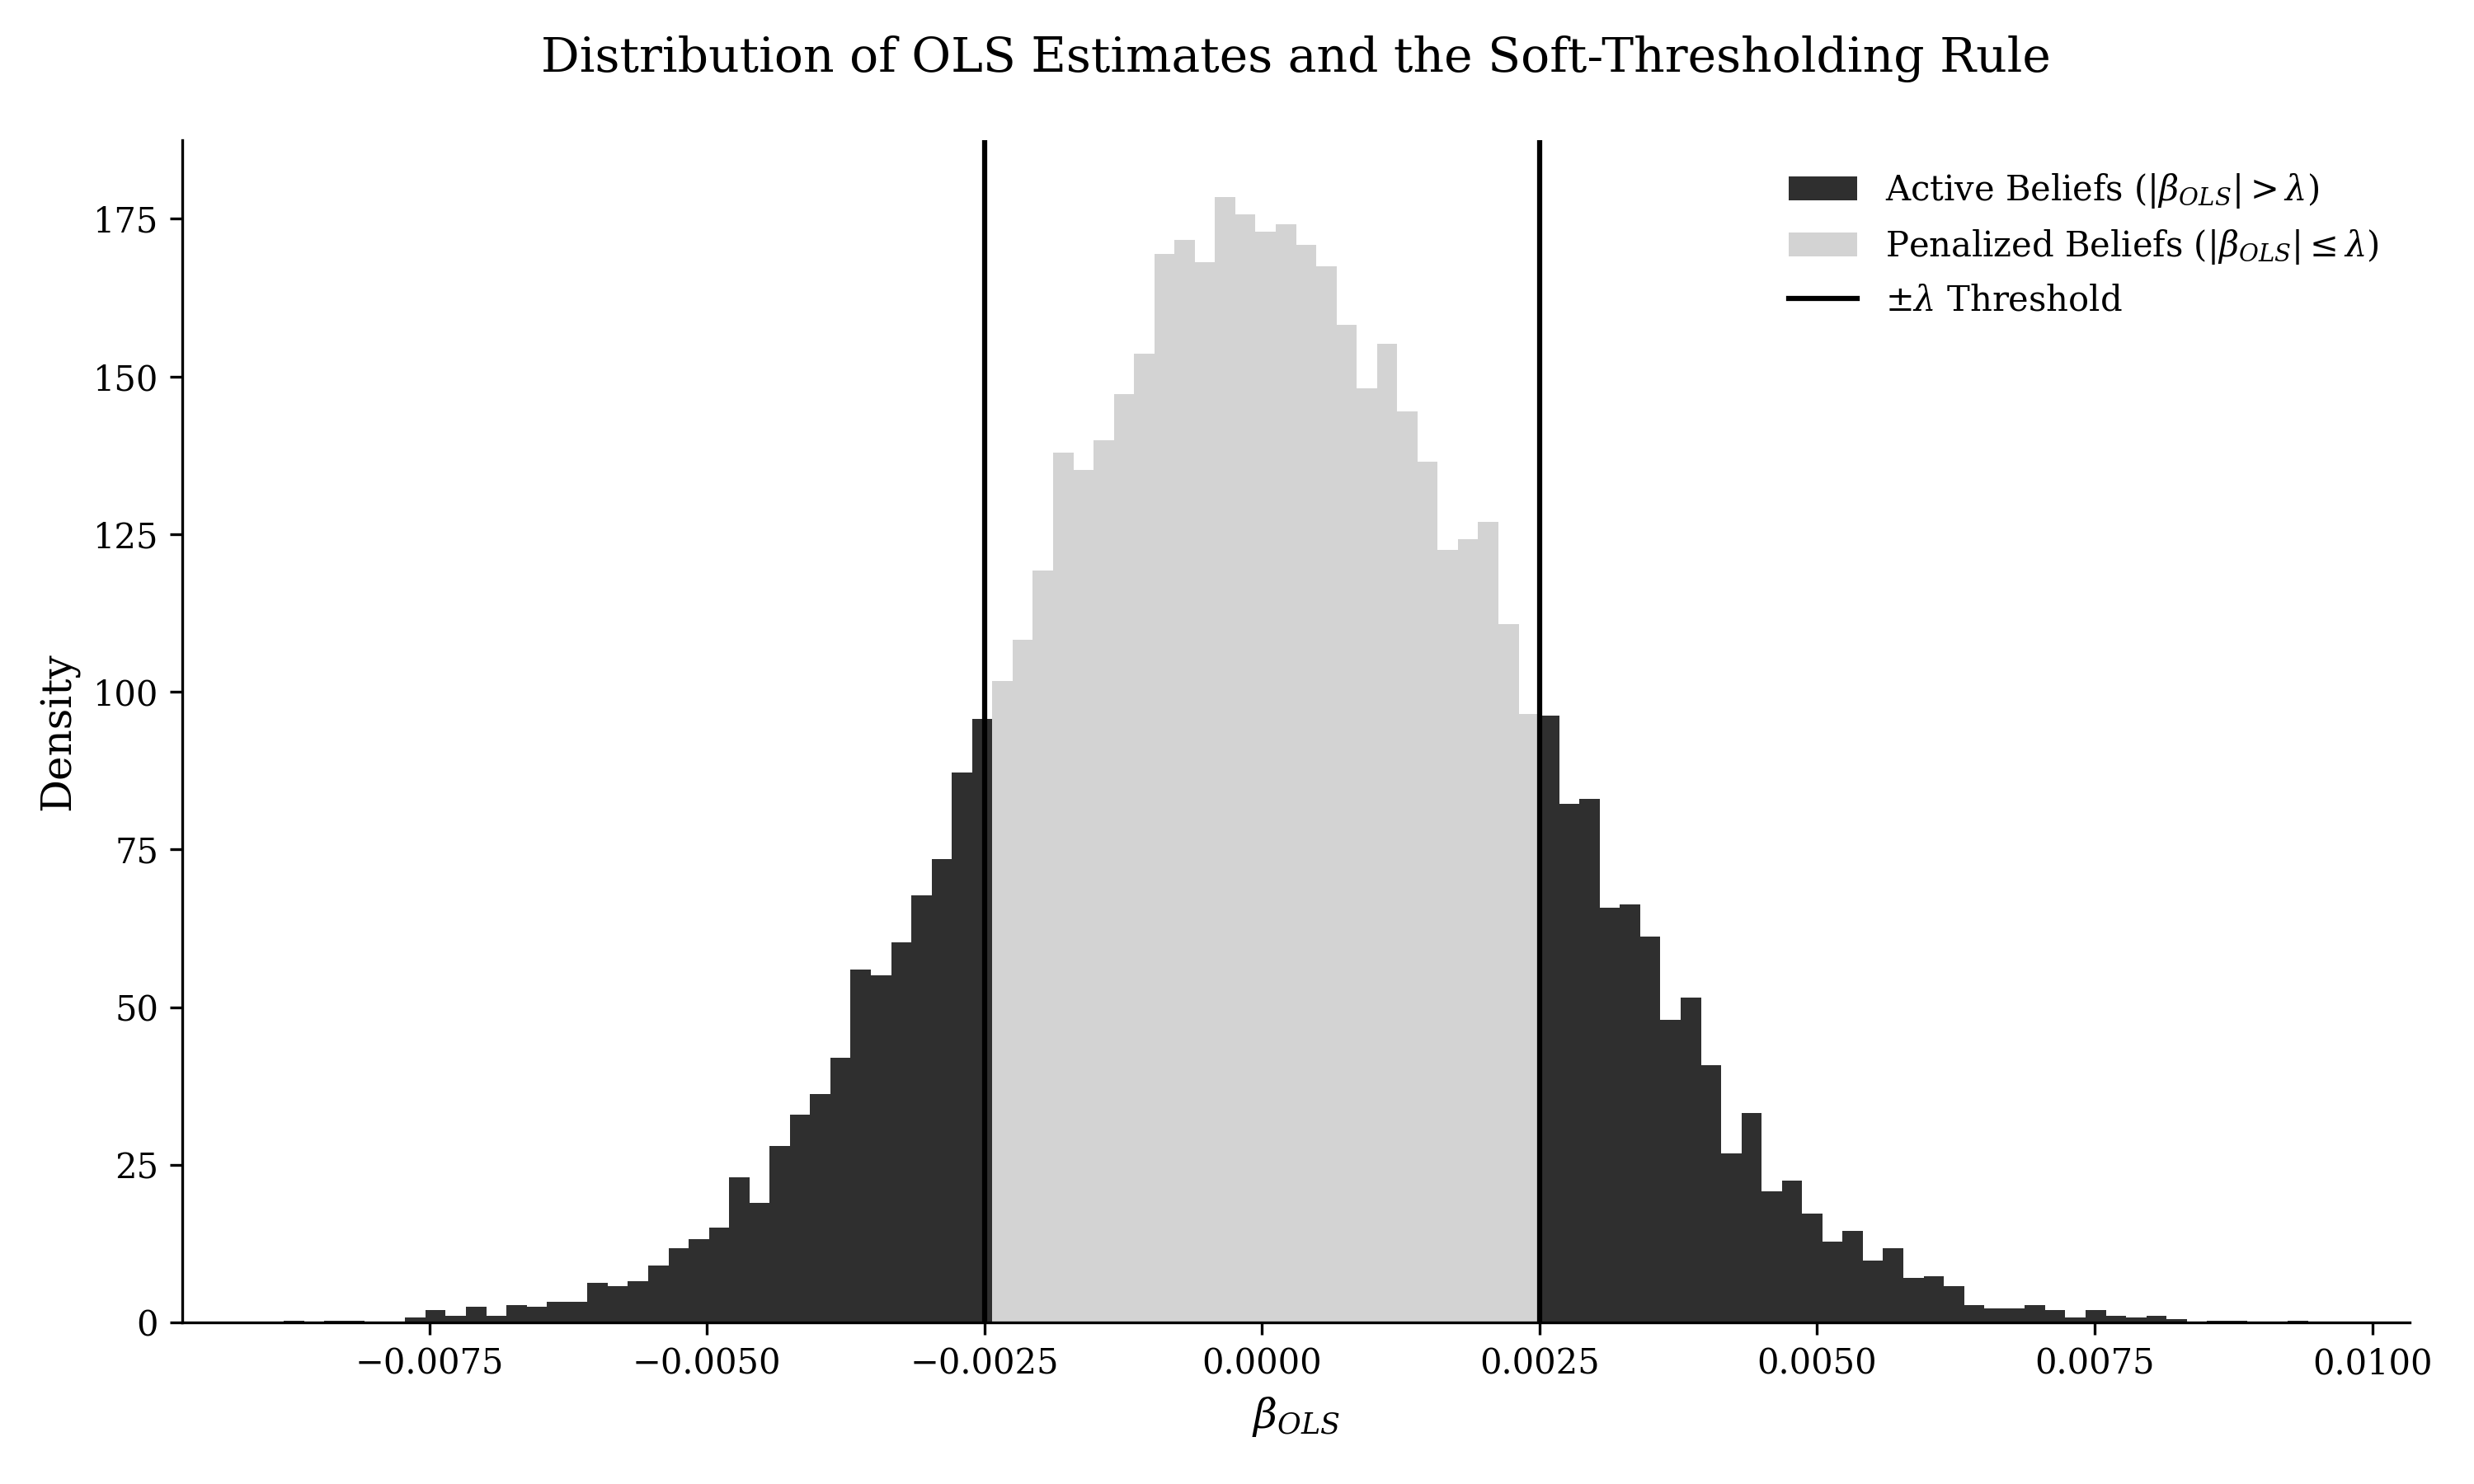
\includegraphics[width=0.5\linewidth]{lasso_threshold_jf_style.png}
    \captionof{figure}{\color{UoCBlue} LASSO Learning Rule. The figure illustrates the soft-thresholding rule applied to OLS coefficients.}
\end{center}

\vspace{0.5cm}
\end{tcolorbox}




\begin{tcolorbox}[colback=white, colframe=UoCBlue, title=Cross-Moment Consistent Equilibrium, toptitle=10pt, bottomtitle=10pt, fonttitle=\bfseries]

\vspace{0.5cm}
\textbf{Misspecification:} Because the ALM is nonlinear and the agents' PLM is linear, learning cannot converge to the true law of motion.

\vspace{0.5cm}
Instead, the economy converges to a Cross-Moment Consistent Equilibrium (CMCE).
\begin{itemize}
    \setlength{\itemsep}{5pt}
    \item The regression coefficients agents estimate match the mathematical projection of actual returns onto the predictors:
    $$ \beta = \frac{\text{Cov}(x_{t}, r_{t+1})}{\text{Var}(x_{t})} $$
    \item We show that the only stable CMCE is $\beta = 0$. 
\end{itemize}

\vspace{0.5cm}
\end{tcolorbox}

\begin{tcolorbox}[colback=white, colframe=UoCBlue, title=The Role of Memory, toptitle=10pt, bottomtitle=10pt, fonttitle=\bfseries]
\vspace{0.5cm}
\begin{itemize}
    \setlength{\itemsep}{5pt}
    \item \textbf{Infinite Memory:} Agents accumulate enough data to perfectly learn that $\beta = 0$.
    \item \textbf{Finite Memory (Our Model):} Agents discount older data. Beliefs constantly fluctuate around the zero-equilibrium due to sampling noise. This finite-sample variance allows LASSO to occasionally select variables, triggering episodic predictability.
\end{itemize}
\vspace{0.5cm}
\end{tcolorbox}


\vspace{0.5cm}
\begin{center}
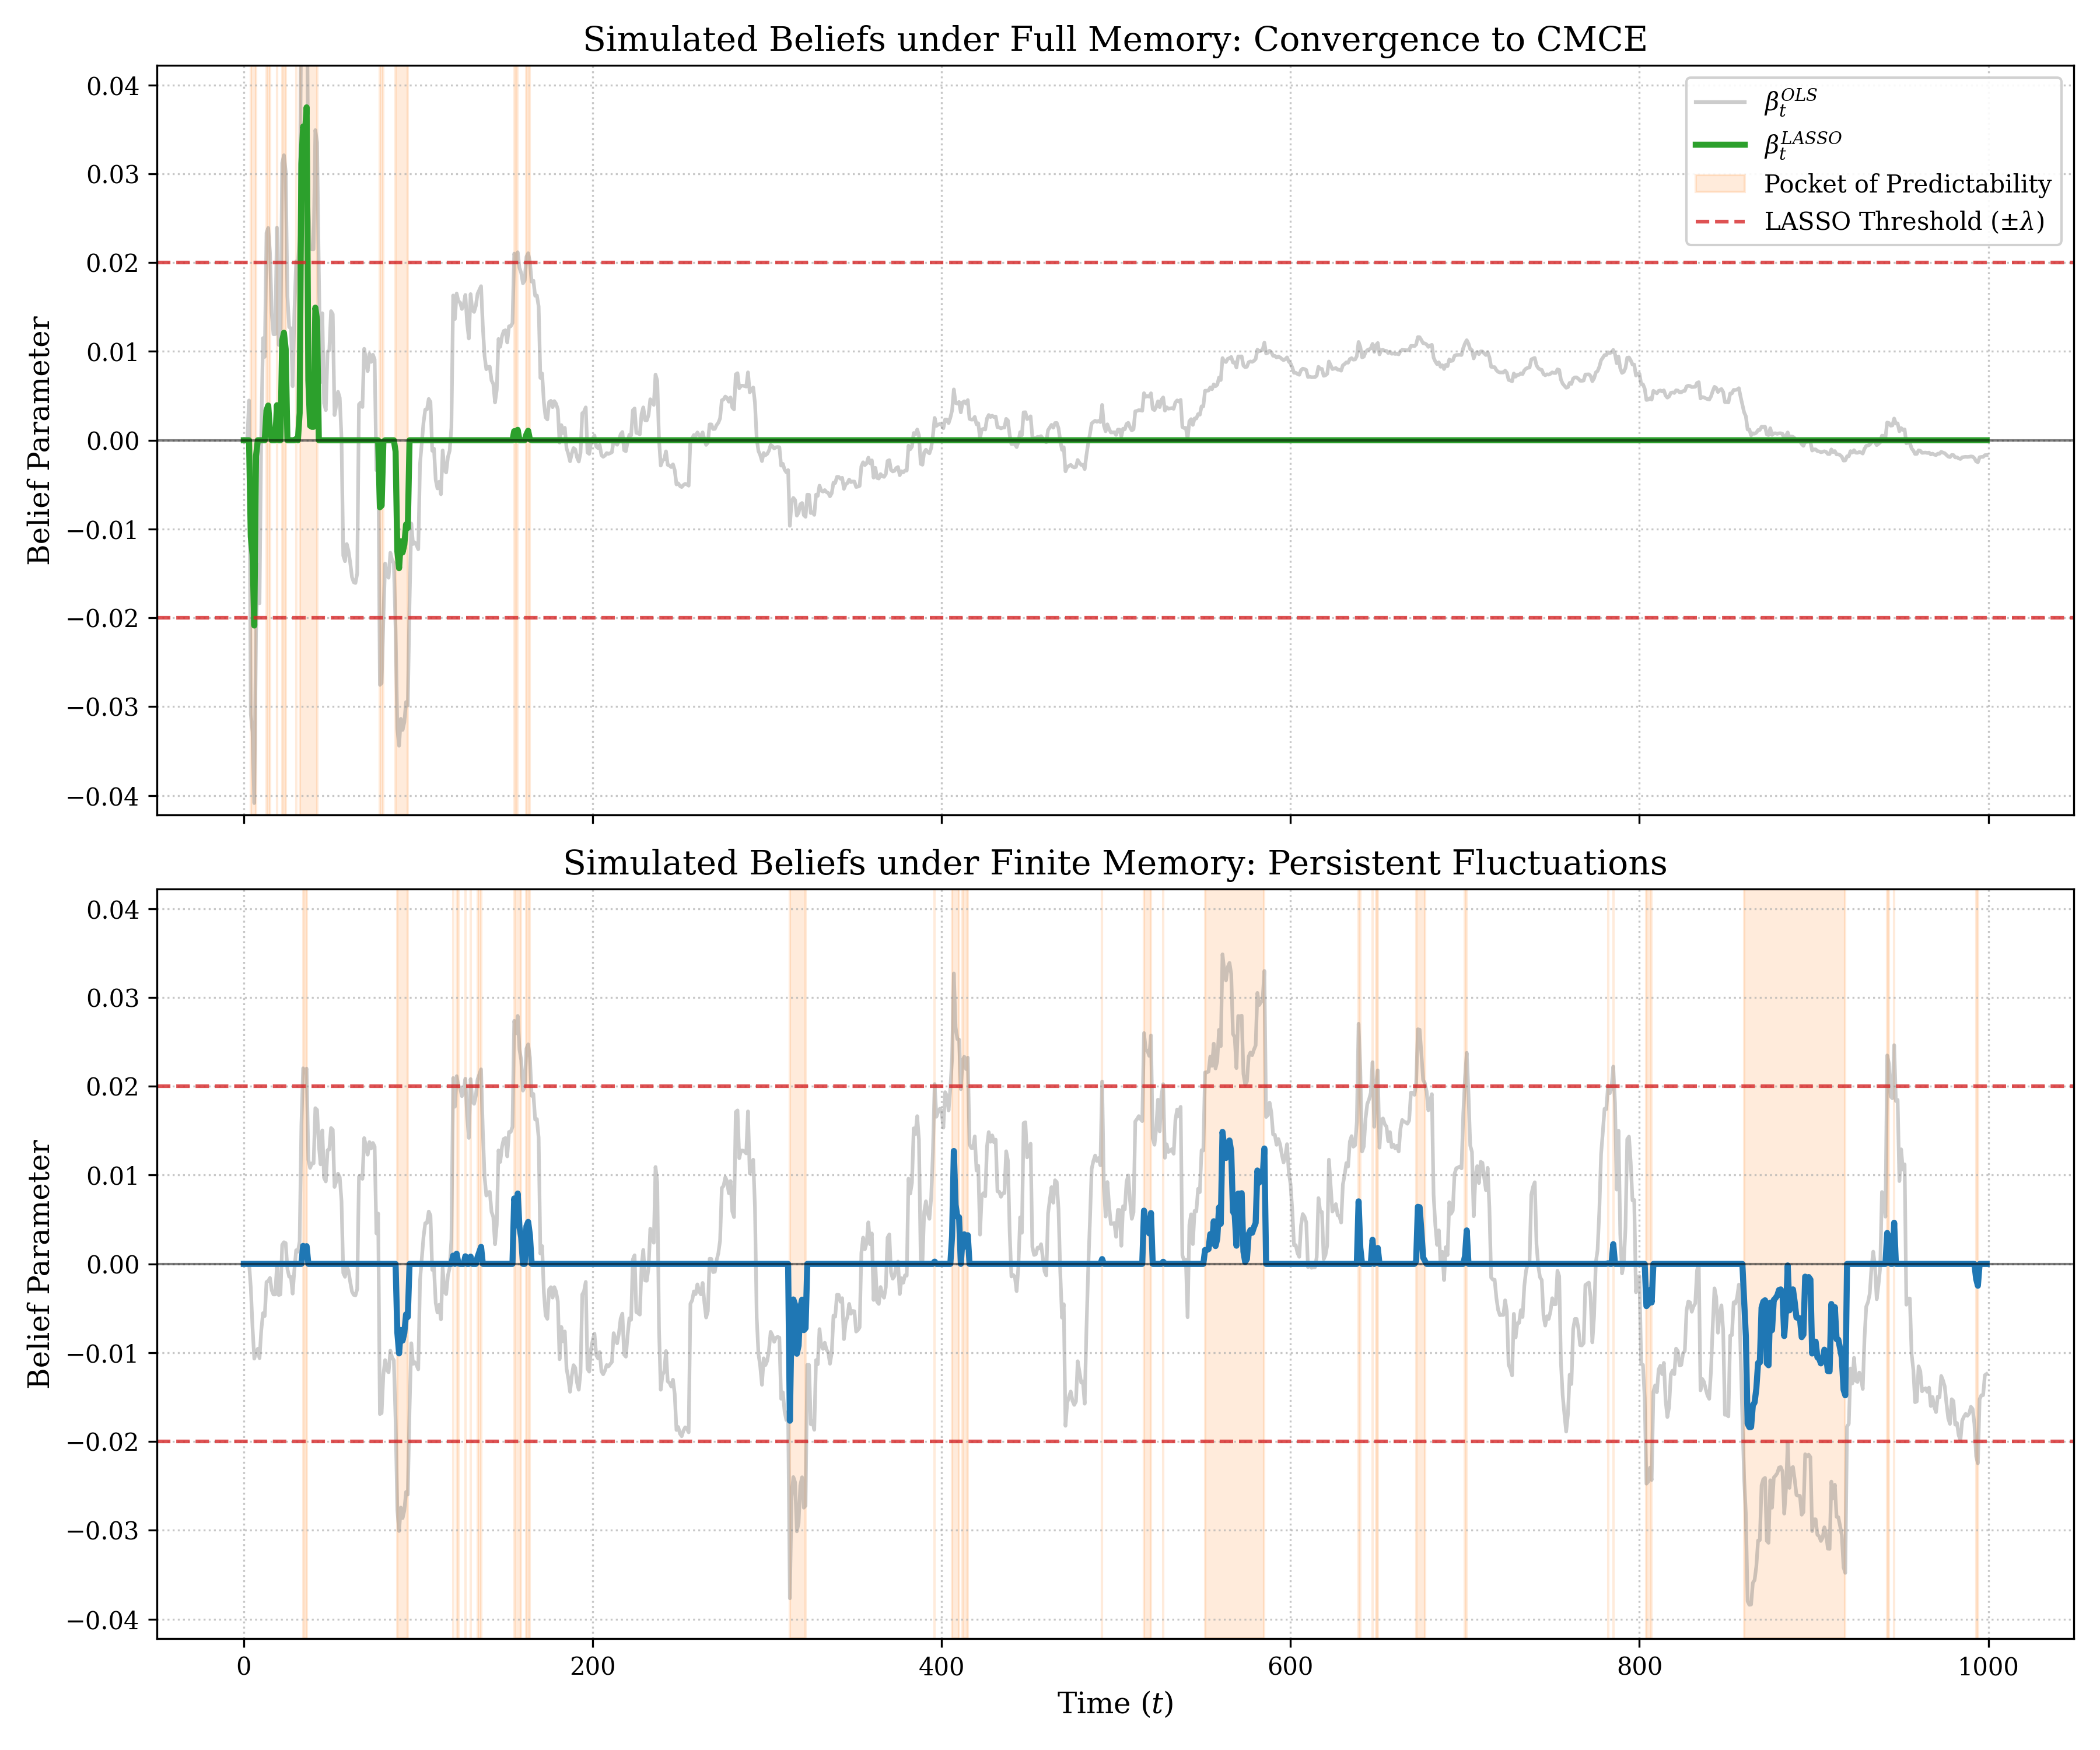
\includegraphics[width=0.8\linewidth]{lasso_comparison.png}
\captionof{figure}{\color{UoCBlue} Simulation of beliefs parameters under LASSO learning with full and finite memory.}
\end{center}



\begin{tcolorbox}[colback=orange!10,colframe=orange,title=Results, toptitle=10pt, bottomtitle=10pt, fonttitle=\bfseries]

\vspace{0.5cm}
\textbf{Pockets of Predictability:} The act of searching for patterns in high-dimensional data endogenously generates short-lived episodes of return predictability.
                                    When predictability emerges, it is highly sparse and concentrated in a small, shifting subset of predictors rather than a stable forecasting relationship.  
                                    This result rationalises recent findings on the sparse and transient nature of return predictability \parencite{chinco2019}. \\

                                    \vspace{0.5cm}

                                    
\textbf{Mechanism:} In finite samples, agents occasionally select predictors by chance. Trading on these perceived signals affects prices, making the predictability temporarily self-fulfilling. As new data arrives, estimates revert to zero, and the predictability disappears.  \\    
\end{tcolorbox}
%----------------------------------------------------------------------------------------
%   EMPIRICAL IMPLEMENTATION & RESULTS
%----------------------------------------------------------------------------------------
\begin{tcolorbox}[presentbox, colframe=UoCBlue, title=Data and Estimation, toptitle=10pt, bottomtitle=10pt, fonttitle=\bfseries]

\vspace{0.5cm}
We estimate the model on 1,620 NYSE stocks using a high-dimensional predictor space of 180 text-based media-attention time series estimated from \textit{Wall Street Journal} articles \parencite{bybee2024}.
In line with the theory, we first estimtate the PLM for each stock and then use the estimated belief paramters to estimate the ALM.
The parameter $\hat{\kappa}$ links investor beliefs to realized returns and we interpret its significance as a statistical test of the model.
We find empirical support for the model in 25\% of all stocks:

\vspace{2cm}

\renewcommand{\arraystretch}{1.4}
\begin{tabularx}{\linewidth}{@{} X c c c @{}} 
\toprule
\textbf{Statistic} & \textbf{Mean} & \textbf{Median} & \textbf{p05 / p95} \\
\midrule
\multicolumn{4}{@{}l}{\textbf{Panel A: Goodness of Fit}} \\
\midrule
PLM In-sample $R^2$ 
  & 0.1056 & 0.0756 & -0.0007 / 0.3161 \\
ALM In-sample $R^2$
  & 0.0016 & 0.0016 & 0.0002 / 0.0033 \\
\midrule
\multicolumn{4}{@{}l}{\textbf{Panel B: Feedback Mechanism}} \\
\midrule
$\hat{\kappa}$ (Feedback Coeff.)
  & 0.6435 & 0.6637 & 0.2337 / 0.9683 \\
$t$-statistic
  & \textbf{9.5058} & \textbf{4.7980} & 2.0958 / 34.4050 \\
\bottomrule
\end{tabularx}

\vspace{0.5cm}
{\small \textit{Note:} The summary statistics are based on a subsample of $N = \text{405}$ stocks (representing \textbf{25\%} of the full sample) that exhibit a statistically significant feedback coefficient ($t > 1.96$).}

\vspace{0.5cm}
\end{tcolorbox}


% %----------------------------------------------------------------------------------------
% %   CONCLUSIONS
% %----------------------------------------------------------------------------------------

% \color{UoCBlue}
% \section*{Future Work}
% \color{Black}
% The model provides a microfoundation for the sparse and episodic nature of return predictability.
% Future work will explore the implications of heterogeneity in memory and the learning rule paramter $\lambda$.

%----------------------------------------------------------------------------------------
%   REFERENCES
%----------------------------------------------------------------------------------------
\color{UoCBlue}
\section*{References}
\color{Black}
\printbibliography[heading=none]
%----------------------------------------------------------------------------------------
%   Acknowledgements
%----------------------------------------------------------------------------------------

\color{UoCGray}
\section*{Acknowledgements}
\color{Black}
Funding from the German Research Foundation (DFG) (EXC 2126/2-390838866).

\end{multicols*}
\end{document}